\paragraph{\trHomotopy{}方法。}\label{sub:homotopy-method}
在\trFloer{}理论中证明\trWellDefinedness{}定理还有另外一种办法。它相当直接
（在历史上也先于\trContinuationMap{}出现），但实现起来在技术上可能颇为棘手。
我们之所以给出这一方法的说明，是因为其内在的重要性，尽管对于眼下的直接
目的而言它并非严格必需。
设对某个带角的\trExactSymplectic\trManifold{} $M$，我们得到了\trFukayaCategory{}
$\scr{F}(M)^{\mathrm{pr},s}$（$s=0,1$）的两个版本。二者应当基于同一个\trStriplikeEnd{}的%
\trUniversal{}选取，从而差异只来自所涉的\trFloerDatum{}与\trPerturbationDatum{}。%
进而我们假设：对每一对 $(L_0,L_1)$，都存在\trFloerDatum{}的一个\trSmooth\trHomotopy
\begin{equation}\label{eq:floer-data-homotopy}
\bigl(H^s_{L_0,L_1},J^s_{L_0,L_1}\bigr),\qquad 0\le s\le 1
\end{equation}
在 $\scr{F}(M)^{\mathrm{pr},0}$ 与 $\scr{F}(M)^{\mathrm{pr},1}$ 所用者之间\trInterpolation。注意：
第一个假设只是技术性的，而第二个假设则相当苛刻，因为它\emph{禁止生灭现象}%
（birth-death phenomena）。为解释这一点，取定 $(L_0,L_1)$ 并从现在起省略下标。
令 $X^s$ 为 $H^s$ 关联的\trHamiltonianVectorField。它还依赖于另一个时间变量
$t\in[0;1]$。以 $\phi^{s,t}$ 表示沿后一方向积分所得的\trHamiltonian\trDiffeomorphism\trFamily，%
即 $\phi^{s,0}=\mathrm{Id}_M$ 且 $\partial\phi^{s,t}/\partial t=X^{s,t}(\phi^{s,t})$。
由于一切\eqref{eq:floer-data-homotopy} 都被假设为\trFloerDatum，诸交集
$\phi^{s,1}(L_0)\cap L_1$ 是\trTransverse{}的，从而交点\trSmooth{}地依赖于 $s$。换个说法：
令 $CF^{\mathrm{pr}}(L_0,L_1)^s$ 为用\eqref{eq:floer-data-homotopy}（对某个
$s\in[0;1]$）定义的\trFloer{}上链群，并令 $\mathscr{C}(L_0,L_1)^s$
为由映射 $y^s\colon[0;1]\to M$ 构成的标准\trGenerator{}集合，其中 $y^s(0)\in L_0$、
$y^s(1)\in L_1$、$dy^s/dt=X^{s,t}(y^s(t))$。类似地，令 $\mathscr{C}(L_0,L_1)^{[0;1]}$
为\trSmooth{}映射 $y\colon[0;1]^2\to M$ 的集合，使得每条限制 $y^s=y(s,\cdot)$
都属于 $\mathscr{C}(L_0,L_1)^s$，并令 $CF^{\mathrm{pr}}(L_0,L_1)^{[0;1]}$ 为该集合%
生成的 $\KK$-\trVectorSpace。那么，限制\trMorphism{}
$\mathscr{C}(L_0,L_1)^{[0;1]}\to\mathscr{C}(L_0,L_1)^s$ 对每个 $s$ 都是\trBijective{}的，于是我们%
有被诱导的\trIsomorphism
\begin{equation}\label{eq:cf-homotopy-identification}
CF^{\mathrm{pr}}(L_0,L_1)^{[0;1]}\cong CF^{\mathrm{pr}}(L_0,L_1)^s.
\end{equation}
指望它们自身就能给出一个 \trAFunctor{}是天真的。毋宁说，需要考虑带一个附加
$s$-参数的\trInhomogeneous\trPseudoholomorphicMap{}的适当\trModuliSpace。
先从一阶构造（即上链层面的映射）开始，它相当透明，可作一般情形的样板。给定
$y_0,y_1\in\mathscr{C}(L_0,L_1)^{[0;1]}$，把 $\scr{M}^*_{\ZZ}(y_0,y_1)^s$ 写作
$\scr{M}^*_{\ZZ}(y_0^s,y_1^s)$，即\trFloerEquation（相对于数据 $(H^s,J^s)$）的非\trStationary{}解%
之\trModuliSpace{}，具极限 $y_0^s,y_1^s$，照常除以\trTranslation。类似地，把
$\scr{M}^*_{\ZZ}(y_0,y_1)^{[0;1]}$ 写作二元组 $(s,u)$ 的空间，其中 $s\in[0;1]$、
$u\in\scr{M}^*_{\ZZ}(y_0^s,y_1^s)$。对 $\nu\ge 1$，我们现引入一个相关的\trModuliSpace{}
$\mathscr{H}^{\nu}(y_0,y_1)^{[0;1]}$，其点为 $\nu$ 元组 $((s_1,u_1),\ldots,(s_{\nu},u_{\nu}))$，
其中 $s_1\le\cdots\le s_{\nu}$，而每个 $u_v\in\scr{M}^*_{\ZZ}(\tilde{y}_{i-1},\tilde{y}_i)^{s_v}$
对某个 $y_0=\tilde{y}_0,\ldots,\tilde{y}_{\nu}=y_1$。可以把 $\mathscr{H}^{\nu}(y_0,y_1)^{[0;1]}$
的元素抽象地看作 2-点\trDisk{}的链，其中每个\trDisk{}都有一个变量 $s_k$ 与之关联，
见\cref{fig:homotopy-chain-discs}。为便于书写，我们形式地规定：$\mathscr{H}^0(y_0,y_1)^{[0;1]}$ 在 $y_0=y_1$
时为一个点，否则为空。
\begin{figure}
\centering
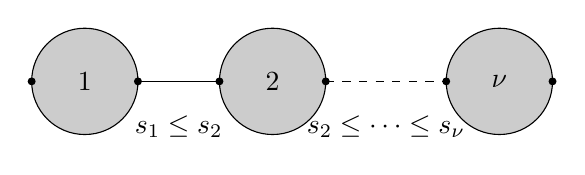
\begin{tikzpicture}[scale=0.9]
\draw[fill=black!20] (0,0) circle (0.75);
\node at (0,0) {$1$};
\fill (-0.75,0) circle (1.6pt);
\fill (0.75,0) circle (1.6pt);
\draw (0.75,0) -- (1.9,0) node[midway,below=9pt] {$s_1\le s_2$};
\draw[fill=black!20] (2.65,0) circle (0.75);
\node at (2.65,0) {$2$};
\fill (1.9,0) circle (1.6pt);
\fill (3.4,0) circle (1.6pt);
\draw[dashed] (3.4,0) -- (5.1,0) node[midway,below=9pt] {$s_2\le\cdots\le s_{\nu}$};
\draw[fill=black!20] (5.85,0) circle (0.75);
\node at (5.85,0) {$\nu$};
\fill (5.1,0) circle (1.6pt);
\fill (6.6,0) circle (1.6pt);
\end{tikzpicture}
\caption{}\label{fig:homotopy-chain-discs}
\end{figure}
可以把我们的构造想成一个经\trParametrization{}的\trModuliSpace{}问题，针对平凡\trFamily{}
$[0;1]\times Z\to[0;1]$，只是与\cref{sub:moduli-spaces-families} 中的设置不同，
与诸端相关联的\trFloerDatum{}随参数 $s$ 变化。尽管如此，基本结构照旧；特别是，
可以对每个 $(s,u)\in\scr{M}^*_{\ZZ}(y_0,y_1)^{[0;1]}$ 关联一个扩张\trLinearization{}算子，
它一如\eqref{eq:extended-linearized-operator} 把附加变量也考虑在内。\trRegularity{}
随之定义为该算子的\trSurjective{}性，并蕴含\trModuliSpace{}的局部\trSmooth{}性。若\trHomotopy{}
\eqref{eq:floer-data-homotopy} 的选取是\trGeneric{}的——我们从此假设如此——则这处处成立。
要看出诸空间 $\mathscr{H}^{\nu}(y_0,y_1)^{[0;1]}$ 性态良好，还需额外证明其%
\trBoundaryFace——即乘积
\begin{equation*}
\prod_{i=1}^{\nu}\scr{M}^*_{\ZZ}(\tilde{y}_{i-1},\tilde{y}_i)^{[0;1]}
\end{equation*}
中由一条或多条形如 $s_i=s_{i+1}$ 的方程切出来的\trSubmanifold——自身也\trRegular。用标准%
\trTransversality{}论证的一个稍加精致的版本，可以证明这能做到，\emph{只要诸}
$(s_i,u_i)$ \emph{两两不同}。幸运的是，该条件在当前语境中自动满足，因为每个 $u_i$
都严格地使 $H^{s_i}$-\trPerturbation{}的\trActionFunctional{}递减。
一个\trEnergy{}论证表明：对充分大的 $\nu$，$\mathscr{H}^{\nu}(y_0,y_1)^{[0;1]}$ 为空。
此外，对固定的 $\nu$，带附加 $s$-参数的一个版本的一个\trGromov\trCompactification{}表明：
$\mathscr{H}^{\nu}(y_0,y_1)^{[0;1]}$ 中只有有限多个\trIsolated{}点。于是我们可以定义一个映射
$\Gamma\colon CF^{\mathrm{pr}}(L_0,L_1)^1\to CF^{\mathrm{pr}}(L_0,L_1)^0$：
\begin{equation}\label{eq:gamma-map}
\Gamma\bigl(y_1^1\bigr)=\sum_{\nu\ge 0}\#\mathscr{H}^{\nu}(y_0,y_1)^{[0;1]}\,y_0^0.
\end{equation}
\begin{lemma}\label{thm:gamma-chain-isomorphism}
$\Gamma$ 是（\trUngraded{}）链\trComplex{}之间的一个\trIsomorphism。
\end{lemma}
证明的想法是直截了当的。把 $\mathscr{H}^{\nu}(y_0,y_1)^{[0;1],1}$ 写作
$\mathscr{H}^{\nu}(y_0,y_1)^{[0;1]}$ 的一维\trConnectedComponent{}之并。这是一个带边%
一维\trManifold，其边界点是使 (i) $s_1=0$、(ii) $s_{\nu}=1$、或 (iii) 对某个 $i$，
$s_{i-1}=s_i$ 的那些点。过渡到\trGromov\trCompactification
$\bar{\mathscr{H}}^{\nu}(y_0,y_1)^{[0;1],1}$ 会添入更多边界点，对应于某个 $u_i$
拆散成一对\trFloer\trTrajectory，这相对于把诸 $\tilde{y}$ 视为变量而言是
$\scr{M}^*_{\ZZ}(\tilde{y}_{i-1},\tilde{y})^{s_i}\times\scr{M}^*_{\ZZ}(\tilde{y},\tilde{y}_i)^{s_i}$
的一个\trIsolated{}点。在对边界点的代数计数中，这些恰好与上述 (iii) 的贡献相消，留下等式
\begin{equation*}
\sum_{\nu\ge 0}\sum_{\tilde{y}}\#\scr{M}^*_{\ZZ}(y_0,\tilde{y})^0\cdot
\#\mathscr{H}^{\nu}(\tilde{y},y_1)^{[0;1]}
+\sum_{\nu\ge 0}\sum_{\tilde{y}}\#\mathscr{H}^{\nu}(y_0,\tilde{y})^{[0;1]}\cdot
\#\scr{M}^*_{\ZZ}(\tilde{y},y_1)^1=0
\end{equation*}
这恰恰是说 $\Gamma$ 是一个\trChainMap。要看它为何是\trIsomorphism，可以大致如下论证。
若诸\trModuliSpace{} $\scr{M}^*_{\ZZ}(y_0,y_1)^{[0;1]}$ 没有\trIsolated{}点，则按定义
$\Gamma=\mathrm{Id}$。在下一个最简单的情形——\trIsolated{}点恰对参数 $s$ 的一个值出现——有
$\Gamma=\mathrm{Id}+(\text{下三角})$，其中第二个被加项相对于由 $A_{H^s}$-作用值给出%
的\trFiltration{}严格递减。最后，利用\eqref{eq:gamma-map} 关于\trHomotopy{}的%
\trComposition{}性态良好这一事实，把一般情形化归为已讨论的情形。沿这些路线的完整%
论证，见下文\cref{thm:homotopy-method-references}中所列文献。
对\trPseudoholomorphic{} $(d{+}1)$ \trPolygon（$d\ge 2$）的类似构造在技术上要更复杂一点。对每一组%
\trExact\trLagrange\trSubmanifold{} $(L_0,\ldots,L_d)$ 选取
\begin{equation}\label{eq:delay-function-choice}
\sigma_{L_0,\ldots,L_d,k}\ \ (1\le k\le d),
\qquad\text{以及}\qquad
\bigl(K^s_{L_0,\ldots,L_d},J^s_{L_0,\ldots,L_d}\bigr)\ \ (0\le s\le 1),
\end{equation}
具如下性质（讨论时将省略下标 $L_0,\ldots,L_d$）。每个 $\sigma_k$ 是一个\trSmooth{}
函数 $\scr{R}^{d+1}\times[0;1]\to[0;1]$，满足 $\sigma_k(r,s)=s$（$s=0,1$）。我们
称这些为\textbf{\trDelayFunction}（delay functions）。诸 $(K^s,J^s)$ 是\trUniversal\trFamily{}
$\scr{S}^{d+1}$ 上\trPerturbationDatum{}的一个\trHomotopy，它在端点 $s=0,1$ 处应化归为
$\scr{F}(M)^{\mathrm{pr},s}$ 所用的数据，并且相对于由诸\trDelayFunction{}确定的
$s$-变量替换与\trFloerDatum{} \eqref{eq:floer-data-homotopy} \trCompatible{}。
显式地说，在每条\trStriplikeEnd{} $\epsilon^{d+1}_k\colon\scr{R}^{d+1}\times\ZZ^{\pm}
\to\scr{S}^{d+1}$ 的像上，我们想要
\begin{equation}\label{eq:perturbation-homotopy-ends}
\begin{split}
(\epsilon^{d+1}_k)^*(K^s,J^s)\qquad\qquad\qquad\qquad\qquad\qquad\quad\\
=\begin{cases}
\bigl(H^s_{L_0,L_d}(t)\,dt,\ J^s_{L_0,L_d}(t)\bigr) & \text{对 } k=0,\\[2pt]
\bigl(H^{\tilde{s}}_{L_{k-1},L_k}(t)\,dt,\ J^{\tilde{s}}_{L_{k-1},L_k}(t)\bigr)
  & \text{对 } k>0\text{，其中 } \tilde{s}=\sigma_k(r,s).
\end{cases}
\end{split}
\end{equation}
这里有一点记号冲突：$t$ 是半无限带 $\ZZ^{\pm}$ 上的第二坐标；然而 $s$
不是第一坐标（它在下面的论证中不起任何作用），而是支配该\trHomotopy{}的变量。
入端与出端处\eqref{eq:perturbation-homotopy-ends} 的\trFloerDatum{}属于一般而言
不同的 $\tilde{s}\neq s$ 值，这一事实影响到把诸\trSurface{}\trGluing{}起来的方式。
现在我们说明如何把\cref{sub:consistent-perturbation-data} 中引入的%
\trPerturbationDatum{}之一致选取的概念\trAdapted{}到当前情形。
设 $T$ 是一棵稳定的 $d$ \trLeafedTree。对每个\trVertex{} $v\in\mathrm{Ve}(T)$，
取定某个 $|v|$ \trPointedDisc{} $S_v$，并令 $r_v\in\scr{R}^{|v|}$ 为相应的模。给这些%
\trDisk{}配备相互\trCompatible{}的\trLagrange\trLabel。再取定 $s\in[0;1]$。于是可以按下面的%
递归规则给每个\trVertex{}关联一个参数值 $s_v\in[0;1]$：第一，若 $v$ 是离根最近的%
\trVertex，则令 $s_v=s$。第二，设 $e$ 是任一内部\trEdge，连接\trVertex{}
$v^-(e)$ 与 $v^+(e)$（我们回忆，\cref{sub:tree-speak} 中诸\trEdge{}的\trOrientation{}背离根），
并设相关联的\trFlag{} $f^-(e)=(v^-(e),e)$ 是按\trCanonical{}次序紧邻 $v^-(e)$ 的第
$k_e$ 个正\trFlag。那么
\begin{equation}\label{eq:recursive-parameter}
s_{v+(e)}=\sigma_{k_e}\bigl(r_{v-(e)},s_{v-(e)}\bigr),
\end{equation}
其中 $\sigma_{k_e}$ 是与 $S_{v-(e)}$ 的诸\trLabel{}（即\trLagrange\trSubmanifold{}的
$|v^-(e)|$ 元组）相关联的诸\trDelayFunction{}之一。现在以某些\trGluingParameter{} $\{\rho_e\}$
把诸 $S_v$ \trGluing{}起来，并令 $r\in\scr{R}^{d+1}$ 为给所得 $(d{+}1)$ \trPointedDisc{} $S$
分类的模点。回顾：$S$ 的诸出向无穷点可与 $T$ 的诸叶等同。若与诸叶相关联的%
\trFlag{}为 $f_{k_1}(v_1),\ldots,f_{k_d}(v_d)$，则我们给这些无穷点配备数
$s^1=\sigma_{k_1}(r_{v_1},s_{v_1}),\ldots,s^d=\sigma_{k_d}(r_{v_d},s_{v_d})\in[0;1]$。
\trConsistency{}条件的第一部分只涉及诸\trDelayFunction，它说：对\trGluingParameter{}的小值，
这些数应当与自然关联于 $S$ 的那些数（即 $\sigma_1(r,s),\ldots,\sigma_d(r,s)$）相合。
等式两侧的\trLagrange\trLabel{}都被我们省略了，但选取是自然的：每个 $S_{v_k}$
都带有\trLagrange\trLabel，因为我们对所有\trVertex{}选取了\trCompatible{}的\trLabel，而 $S$
经由\trGluing{}过程从它们承袭\trLabel。接着，给每个 $S_v$ 配备时刻 $s_v$ 的%
\trPerturbationDatum{} \eqref{eq:delay-function-choice}。条件
\eqref{eq:perturbation-homotopy-ends} 与\eqref{eq:recursive-parameter}
合在一起保证：这些数据在相应的出端\trStriplikeEnd{}上有相同的行为，从而可以\trGluing
成 $S$ 上的一个\trPerturbationDatum。另一方面，也可以给同一\trDisk{}配备经分类\trIsomorphism%
$S\cong\scr{S}^{d+1}_r$ 从\eqref{eq:delay-function-choice} \trPullback{}而来的%
\trPerturbationDatum。\trConsistency{}条件要求这两个数据之间有与
\cref{sub:consistent-perturbation-data} 中相同的关系：对\trGluingParameter{}的小值在 $S$
的薄部上相等，而在厚部上\trAsymptotic{}相合（后者借助\trUniversal\trFamily{}的%
\trPartialCompactification{}来定义）。
在做出了上述意义下一致的一组\eqref{eq:delay-function-choice} 选取之后，便可以
引入相关的\trModuliSpace。给定 $(L_0,\ldots,L_d)$ 与 $y_0\in\mathscr{C}(L_0,L_d)^{[0;1]}$、
$y_k\in\mathscr{C}(L_{k-1},L_k)^{[0;1]}$，令 $\scr{M}^{d+1}(y_0,\ldots,y_d)^{[0;1]}$
为三元组 $(r,s,u)$ 构成的空间，其中 $r\in\scr{R}^{d+1}$、$s\in[0;1]$，而
$u\colon\scr{S}^{d+1}_r\to M$ 是 $S$ 上带\trPerturbationDatum{}
\eqref{eq:delay-function-choice} 的\trInhomogeneous\trPseudoholomorphicMap{}方程的一个解，其极限
为：入端\trStriplikeEnd{}上的 $y_0^s$，以及诸出端上的 $y_k^{\tilde{s}}$（其中
$\tilde{s}=\sigma_{L_0,\ldots,L_d,k}(r,s)$）。与先前考察的
$\mathscr{H}^{\nu}(y_0,\ldots,y_d)^{[0;1]}$ 平行，还有另一族密切相关的\trModuliSpace{}
$\mathscr{I}^T(y_0,\ldots,y_d)^{[0;1]}$。其定义部分地类似于
\cref{sub:compactness} 中所讨论的\trCompactification；我们将从那里借用一些记号。取定一棵半稳定的
$d$ \trLeafedTree{}$T$。$\mathscr{I}^T(y_0,\ldots,y_d)^{[0;1]}$ 中的一点由如下数据组成：
\begin{itemize}
\item 对每个满足 $|v|\ge 3$ 的\trVertex{}，一个 $r_v\in\scr{R}^{|v|}$，从而一个
$|v|$ \trPointedDisc{} $S_v$。对其余\trVertex，取 $S_v=\ZZ$。
\end{itemize}
有一种唯一的方式给诸 $S_v$ 配备\trCompatible\trLagrange\trLabel，使得\trGluing{}而成的
$(d{+}1)$ \trPointedDisc{}上被诱导的\trLabel{}正是给定的诸 $L_k$。做完这一步后，下一组
数据是：
\begin{itemize}
\item 对每个 $v$ 一个数 $s_v\in[0;1]$，满足\eqref{eq:recursive-parameter}
的一个不等式版本。即：对每条内部\trEdge{} $e$，
\begin{equation}\label{eq:inequality-parameter}
s_{v+(e)}\ge
\begin{cases}
\sigma_k\bigl(r_{v-(e)},s_{v-(e)}\bigr) & \text{若 } |v^-(e)|\ge 3,\\
s_{v-(e)} & \text{若 } |v^-(e)|=2.
\end{cases}
\end{equation}
\end{itemize}
接着，回顾在此情形每个\trFlag{} $f$ 都关联着一对 $(L_{f,0},L_{f,1})$
\trLagrange\trSubmanifold。
\begin{itemize}
\item 对每个 $f$，我们要指派一个 $\tilde{y}_f\in\mathscr{C}(L_{f,0},L_{f,1})^{[0;1]}$，%
受以下条件约束。若 $f$ 是与 $T$ 的根相关联的唯一\trFlag，则 $\tilde{y}_f=y_0$。
类似地，对与诸叶相关联的 $d$ 条\trFlag，诸 $\tilde{y}_f$ 将是 $y_1,\ldots,y_d$。
而若 $f^{\pm}(e)$ 是属于某条内部\trEdge{}的两条\trFlag，则
$\tilde{y}_{f^-(e)}=\tilde{y}_{f^+(e)}$。
\item 最后，对每个 $v$ 一个映射 $u_v\colon S_v\to M$：当 $|v|=2$ 时它是\eqref{eq:floer-equation}
的非\trStationary{}解，当 $|v|\ge 3$ 时它是\eqref{eq:inhomogeneous-equation} 的解；相关的%
\trFloerDatum{}与\trPerturbationDatum{}分别由\eqref{eq:floer-data-homotopy} 与
\eqref{eq:delay-function-choice} 给出，取 $s=s_v$；而在诸\trStriplikeEnd{}上的极限值
应当是关联于 $v$ 周围诸\trFlag{} $f$ 的诸 $\tilde{y}_f$。换个说法：
\begin{equation*}
\begin{cases}
(s_v,u_v)\in\scr{M}^*_{\ZZ}\bigl(\tilde{y}_{f_0(v)},\tilde{y}_{f_1(v)}\bigr)^{[0;1]}
  & \text{对 } |v|=2,\\
(r_v,s_v,u_v)\in\scr{M}^{d+1}\bigl(\tilde{y}_{f_0(v)},\ldots,\tilde{y}_{f_d(v)}\bigr)^{[0;1]}
  & \text{对 } |v|\ge 3.
\end{cases}
\end{equation*}
\end{itemize}
图 10.3 展示了诸\trSurface{} $S_v$ 及其\trLagrange\trLabel{}的示意图，以及诸 $s_v$
之间所得的不等式。照例，仅相差每个非稳定\trConnectedComponent{} $S_v\cong\ZZ$
的一个\trTranslation{}的族 $\{u_v\colon S_v\to M\}$ 将被视为相同。
\begin{figure}
\centering
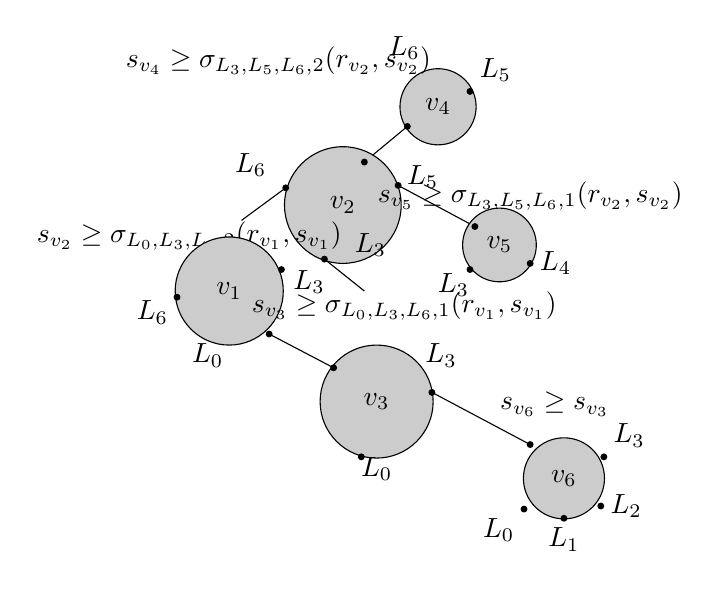
\begin{tikzpicture}[scale=0.78]
\draw[fill=black!20] (4.1,7.6) circle (0.62);
\node at (4.1,7.6) {$v_4$};
\fill (4.62,7.85) circle (1.6pt) node[above right] {$L_5$};
\fill (3.6,7.28) circle (1.6pt);
\node at (3.55,8.55) {$L_6$};
\draw (3.6,7.28) -- (2.9,6.7);
\node at (1.5,8.35) {$s_{v_4}\ge\sigma_{L_3,L_5,L_6,2}(r_{v_2},s_{v_2})$};
\draw[fill=black!20] (2.55,6.0) circle (0.95);
\node at (2.55,6.0) {$v_2$};
\fill (2.9,6.7) circle (1.6pt);
\fill (3.45,6.32) circle (1.6pt) node[right] {};
\fill (1.62,6.28) circle (1.6pt);
\fill (2.25,5.12) circle (1.6pt);
\node at (1.05,6.65) {$L_6$};
\node at (3.85,6.45) {$L_5$};
\node at (3.0,5.35) {$L_3$};
\draw (3.45,6.32) -- (4.7,5.65);
\draw (1.62,6.28) -- (0.9,5.75);
\draw (2.25,5.12) -- (2.9,4.6);
\node at (5.6,6.15) {$s_{v_5}\ge\sigma_{L_3,L_5,L_6,1}(r_{v_2},s_{v_2})$};
\draw[fill=black!20] (5.1,5.35) circle (0.6);
\node at (5.1,5.35) {$v_5$};
\fill (4.7,5.65) circle (1.6pt);
\fill (5.6,5.05) circle (1.6pt) node[right] {$L_4$};
\fill (4.62,4.95) circle (1.6pt);
\node at (4.35,4.7) {$L_3$};
\node at (0.05,5.5) {$s_{v_2}\ge\sigma_{L_0,L_3,L_6,2}(r_{v_1},s_{v_1})$};
\draw[fill=black!20] (0.7,4.6) circle (0.88);
\node at (0.7,4.6) {$v_1$};
\fill (0.9,5.75) circle (0.01pt);
\fill (1.55,4.95) circle (1.6pt);
\fill (1.35,3.9) circle (1.6pt);
\fill (-0.15,4.5) circle (1.6pt);
\node at (-0.55,4.25) {$L_6$};
\node at (2.0,4.75) {$L_3$};
\node at (0.35,3.55) {$L_0$};
\draw (1.35,3.9) -- (2.4,3.35);
\node at (3.55,4.35) {$s_{v_3}\ge\sigma_{L_0,L_3,L_6,1}(r_{v_1},s_{v_1})$};
\draw[fill=black!20] (3.1,2.8) circle (0.92);
\node at (3.1,2.8) {$v_3$};
\fill (2.4,3.35) circle (1.6pt);
\fill (4.0,2.95) circle (1.6pt);
\fill (2.85,1.9) circle (1.6pt);
\node at (4.15,3.55) {$L_3$};
\node at (3.1,1.7) {$L_0$};
\draw (4.0,2.95) -- (5.6,2.1);
\node at (6.0,2.75) {$s_{v_6}\ge s_{v_3}$};
\draw[fill=black!20] (6.15,1.55) circle (0.66);
\node at (6.15,1.55) {$v_6$};
\fill (5.6,2.1) circle (1.6pt);
\fill (6.8,1.9) circle (1.6pt) node[above right] {$L_3$};
\fill (6.75,1.1) circle (1.6pt) node[right] {$L_2$};
\fill (5.5,1.05) circle (1.6pt) node[below left] {$L_0$};
\fill (6.15,0.9) circle (1.6pt) node[below] {$L_1$};
\end{tikzpicture}
\caption{}\label{fig:homotopy-tree-surfaces}
\end{figure}
设\eqref{eq:delay-function-choice} 中的选取足够\trGeneric，则类比
\eqref{eq:gamma-map} 可定义多重\trLinear{}映射
\begin{equation}\label{eq:higher-homotopy-maps}
\begin{split}
\mathscr{G}^d\colon CF^{\mathrm{pr}}(L_{d-1},L_d)^1\otimes\cdots\otimes
CF^{\mathrm{pr}}(L_0,L_1)^1&\longrightarrow CF^{\mathrm{pr}}(L_0,L_d)^0,\\
\mathscr{G}^d\bigl(y_d^1,\ldots,y_1^1\bigr)
&=\sum_T\#\mathscr{I}^T(y_0,\ldots,y_d)^{[0;1]}\,y_0^0.
\end{split}
\end{equation}
\begin{proposition}\label{thm:homotopy-afunctor}
映射 $\mathscr{G}^1=\Gamma$（\eqref{eq:gamma-map}）与各高阶项 $\mathscr{G}^d$
（\eqref{eq:higher-homotopy-maps}）构成一个（\trUngraded{}的）\trAFunctor
\begin{equation*}
\mathscr{G}\colon\scr{F}(M)^{\mathrm{pr},1}\longrightarrow\scr{F}(M)^{\mathrm{pr},0}.
\end{equation*}
\end{proposition}
注意，由\cref{thm:gamma-chain-isomorphism}，诸\trLinear{}部分 $\mathscr{G}^1$ 都是%
\trIsomorphism（若经\eqref{eq:cf-homotopy-identification} 等同诸 $CF^{\mathrm{pr}}(L_0,L_1)^s$
（$s=0,1$），则 $\mathscr{G}$ 是\cref{sub:formal-diffeomorphisms} 意义下的一个%
\trFormalDiffeomorphism）。特别地，$\scr{F}(M)^{\mathrm{pr},0}$ 与
$\scr{F}(M)^{\mathrm{pr},1}$ 是相互\trQuasiisomorphic{}的 \trAinfty-\trCategory。
\cref{thm:homotopy-afunctor}的证明策略与\cref{thm:gamma-chain-isomorphism}基本相同。
一维\trModuliSpace{} $\mathscr{I}^T(y_0,\ldots,y_d)^{[0;1],1}$ 的边界点出现在：
(i) 离根最近的\trVertex{}处 $s_v=0$；(ii) 离诸叶最近的某个\trVertex{}处 $s_v=1$；
或 (iii) \eqref{eq:inequality-parameter} 之一取等号。在前两种情形，如图 10.4 所示
把树分成几块，便可断言相关的代数贡献恰是 \trAinfty-\trFunctor{}方程
\eqref{eq:afunctor-equations} 中的两项。来自 (iii) 的贡献再次与\trGromov\trCompactification{}所引入的
附加点相消。当然，这一形式概要并不构成一个完整的证明。不过，其中大部分分析并不比
定义\trFukayaCategory{}所用的分析精致多少。因此我们将只限于讨论\trTransversality{}%
问题的一个特定方面，即引入诸\trDelayFunction{}的动机所在。为把这一点看得更清楚，
我们暂时把自己限制在平凡\trDelayFunction{} $\sigma_k(r,s)=s$ 的情形。
\begin{figure}
\centering
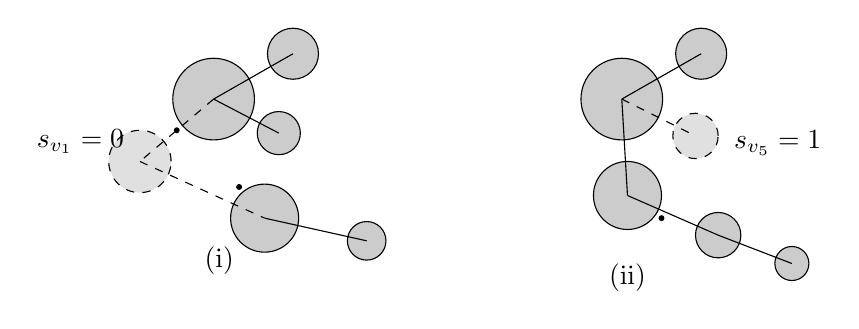
\begin{tikzpicture}[scale=0.72]
\begin{scope}
\draw[fill=black!20] (2.2,2.5) circle (0.72);
\draw[fill=black!20] (3.6,3.3) circle (0.45);
\draw[fill=black!20] (3.35,1.9) circle (0.38);
\draw[fill=black!20] (3.1,0.4) circle (0.6);
\draw[fill=black!20] (4.9,0.0) circle (0.34);
\draw[fill=black!12,dashed] (0.9,1.4) circle (0.55);
\draw (2.2,2.5) -- (3.6,3.3);
\draw (2.2,2.5) -- (3.35,1.9);
\draw[dashed] (2.2,2.5) -- (0.9,1.4);
\draw[dashed] (0.9,1.4) -- (3.1,0.4);
\draw (3.1,0.4) -- (4.9,0.0);
\fill (1.55,1.95) circle (1.5pt);
\fill (2.65,0.95) circle (1.5pt);
\node at (-0.15,1.75) {$s_{v_1}=0$};
\node at (2.3,-0.35) {(i)};
\end{scope}
\begin{scope}[shift={(7.2,0)}]
\draw[fill=black!20] (2.2,2.5) circle (0.72);
\draw[fill=black!20] (3.6,3.3) circle (0.45);
\draw[fill=black!12,dashed] (3.5,1.85) circle (0.4);
\draw[fill=black!20] (2.3,0.8) circle (0.6);
\draw[fill=black!20] (3.9,0.1) circle (0.4);
\draw[fill=black!20] (5.2,-0.4) circle (0.3);
\draw (2.2,2.5) -- (3.6,3.3);
\draw[dashed] (2.2,2.5) -- (3.5,1.85);
\draw (2.2,2.5) -- (2.3,0.8);
\draw (2.3,0.8) -- (3.9,0.1);
\draw (3.9,0.1) -- (5.2,-0.4);
\fill (2.9,0.4) circle (1.5pt);
\node at (4.95,1.72) {$s_{v_5}=1$};
\node at (2.3,-0.65) {(ii)};
\end{scope}
\end{tikzpicture}
\caption{}\label{fig:homotopy-tree-splits}
\end{figure}
首先，可以\trGeneric{}地选取\eqref{eq:delay-function-choice} 中的%
\trPerturbationDatum，使得诸空间 $\scr{M}^{d+1}(y_0,\ldots,y_d)^{[0;1]}$ 都\trRegular。
剩下的问题是保证 $\mathscr{I}^T(y_0,\ldots,y_d)^{[0;1]}$ 的诸\trBoundaryFace——
它们是乘积
\begin{equation}\label{eq:boundary-face-products}
\prod_{v\in\mathrm{Ve}(T)}\scr{M}^{|v|}\bigl(\tilde{y}_{f_0(v)},\ldots,
\tilde{y}_{f_{|v|-1}(v)}\bigr)^{[0;1]}
\end{equation}
中由等式
\begin{equation}\label{eq:parameter-equality}
s_{v+(e)}=s_{v-(e)}.
\end{equation}
切出来的子集——仍然\trRegular。好在只需考虑维数 $\le 1$ 的\trModuliSpace，这使事情
稍微容易些。例如，在零维情形，所要做出的陈述是：若
$\{u_v\colon S_v\to M\}\in\mathscr{I}^T(y_0,\ldots,y_d)^{[0;1]}$ 使得每个
$(r_v,s_v,u_v)$ 都是\eqref{eq:boundary-face-products} 中相应因子的\trIsolated{}点，则
\eqref{eq:parameter-equality} 对任何\trEdge{} $e$ 都绝不成立。标准%
\trTransversality{}论证表明，这可以经\trPerturbationDatum{}的一个\trGeneric{}选取
达到，\emph{除非}与相关\trVertex{}相关联的两个映射相同：
\begin{equation}\label{eq:pathological-coincidence}
S_{v^-(e)}\cong S_{v^+(e)}
\quad\text{且}\quad
u_{v^-(e)}=u_{v^+(e)}.
\end{equation}
不幸的是，与先前讨论映射 $\Gamma$ 时的可比较之点不同，这一残余情形不可能被排除：
存在在入端上的极限与在（一条或几条）出端上的极限相同的\trRegular\trPseudoholomorphic\trPolygon
$(d{+}1)$ 边形。现在允许非平凡的\trDelayFunction{}：此时考察的不再是
\eqref{eq:parameter-equality}，而是让\eqref{eq:inequality-parameter} 中的一部分
不等式变成等式。经\trGeneric{}选取，下述成立：\emph{若 $(r,s,u)$ 是某个\trModuliSpace{}
$\scr{M}^{d+1}(y_0,\ldots,y_d)^{[0;1]}$（$d\ge 2$）的\trIsolated{}点，则诸\trDelayFunction{}
满足 $\sigma_k(r,s)\neq s$（对一切 $k=1,\ldots,d$）。}这一条件显然排除了
\eqref{eq:pathological-coincidence} 那样的病态行为，从而使人得以完成%
\trTransversality{}论证。对一维\trModuliSpace{}的平行考虑，我们略去不表——它们只是
稍微更费些事而已。
\begin{remark}\label{thm:homotopy-method-references}
\trFloerHomology{}的\trHomotopy{}方法已见于\trFloer{}的原始论文 [44]。到\trFukayaCategory{}%
的推广遵循\trFukaya--\trOh--\trOhta--\trOno{} [60, Theorem 15.19]，只是我们把虚拟\trPerturbation{}理论
换成了一个更显式的\trTransversality{}论证。附带指出：在非\trExact{}情形下处理%
\trFloerHomology{}时，\trTransversality{}问题会变得更严重，而且迄今只找到了间接的解法
（见 [94]，或 [78]——Morse--Novikov 理论的模型情形）。
\end{remark}
